\renewcommand{\thechapter}{8}
\chapter{Conclusions and Future Plans}
\label{ch:Conclusions}

This work has presented a wide-ranging upgrade to the scintillation waveform analysis of EXO-200.  The result has been a 21\% improvement in the single-site energy resolution at the $Q$-value, from 1.94\% to 1.53\% $\sigma/E$.  We strengthen the half-life limit of $\beta\beta 0\nu$ decay for this analysis by 11\%, corresponding to a 6\% stronger limit on the Majorana neutrino mass.  Separate background fits to the denoised and undenoised data indicate that the $2\sigma$ region of interest background is reduced 32\% by denoising, corresponding to a mean sensitivity which is strengthened by 17\% and a mean sensitivity for the Majorana mass which is 9\% lower than could be achieved without denoising.

\begin{figure}
\begin{center}
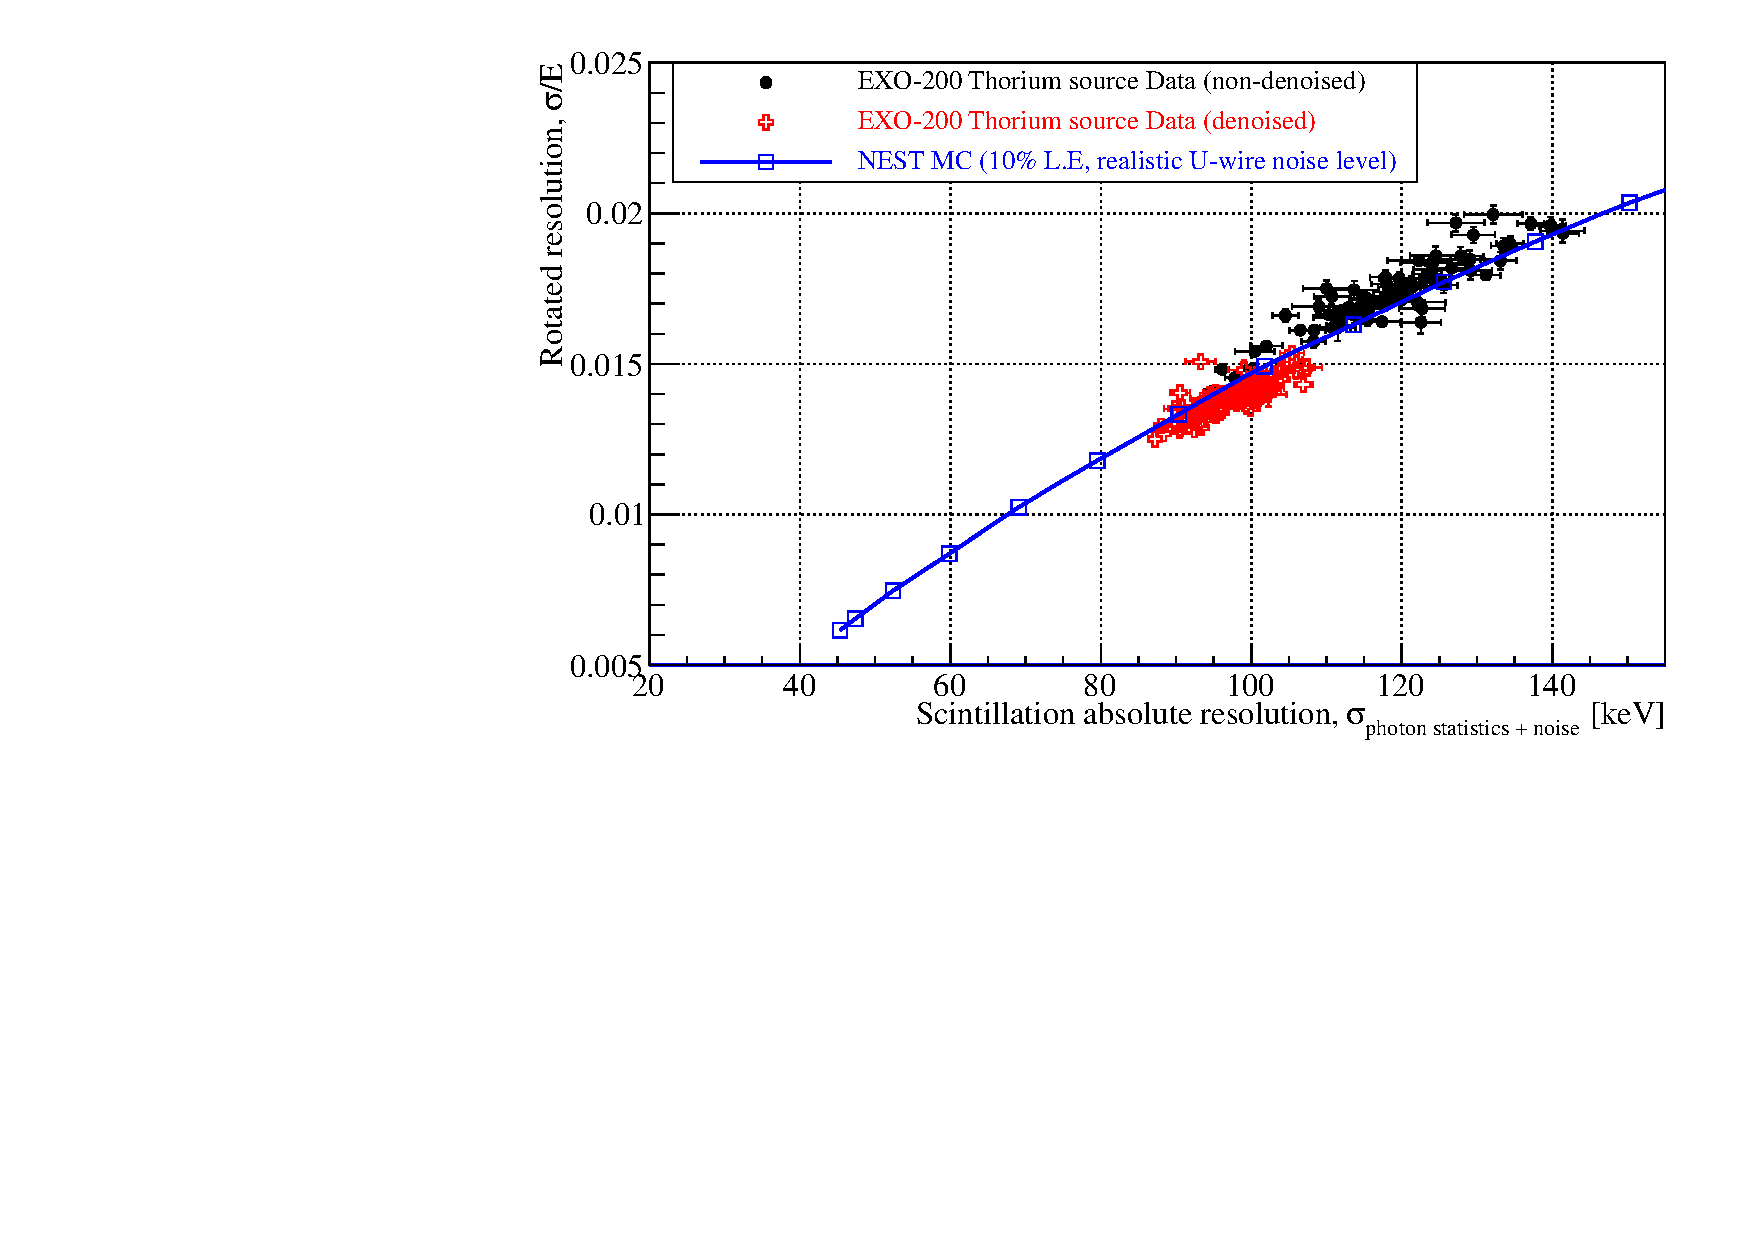
\includegraphics[keepaspectratio=true,width=\textwidth]{resoDataMC_800eRMSInIonization_Comp.pdf}
\end{center}
\renewcommand{\baselinestretch}{1}
\small\normalsize
\begin{quote}
\caption{NEST simulation software has been used to estimate how the rotated energy resolution at 2615 keV (vertical axis) depends on the scintillation-only resolution at 2615 keV (horizontal axis); this theoretical estimate is shown in blue, as applicable to the EXO-200 detector with fixed electric field.  Black points indicate measurements from thorium source runs without denoising; red points indicate measurements from thorium runs with denoising.  Figure provided by Liangjian Wen using NEST software~\cite{NESTpaper}.}
\label{fig:ScintillationVsOverallResolution_NEST}
\end{quote}
\end{figure}
\renewcommand{\baselinestretch}{2}
\small\normalsize

One question which must be asked is whether there is any room for further improvement in the energy resolution.  Figure~\ref{fig:ScintillationVsOverallResolution_NEST} shows simulations of the relationship between scintillation-only resolution and rotated energy resolution.  Points indicate the resolutions measured from denoised and non-denoised data; we can see that the model agrees well with both sets of data.  Based on these simulations, it is clear that further improvements to the scintillation resolution will indeed have a significant impact on the overall resolution of EXO-200; projections from figure~\ref{fig:BackgroundVsResolution} indicate that $^{232}$Th and $^{137}$Xe backgrounds can continue to be significantly reduced by resolution improvements, so these attempts are indeed worthwhile.

We have noted in section~\ref{sec:DenoisingInPractice} that the parameters used for this denoising are not optimal, and that preliminary studies indicate roughly 0.05 percentage points can be gained in overall energy resolution at 2615 keV with an up-to-date set of denoising parameters.  This issue is straightforward to address, and the next processing of our dataset will incorporate it.

Beyond this improvement, we have described in section~\ref{sec:ResultEnergyLight} that the denoised scintillation peak position displays a large position dependence which cannot be fully calibrated in downstream analysis.  The effect of this feature is to dilute our resolution improvements.  Although the cause of this position dependence is not fully understood, we believe that it originates in the lightmap because the lightmap is the input to denoising which encodes position-dependent yield information; one preliminary theory is that the discrepancy between 1-wire and 2-wire charge peak positions described in section~\ref{sec:ResultEnergyCharge} leads to a bias in event selection for the lightmap.  We believe that this issue can be addressed with further investigation and will lead to additional significant improvements in resolution.

The most exciting improvement in resolution may come not from offline analysis but from planned electronics upgrades.  There are indications that the source of electronic noise in the APDs is now understood and can be fixed in hardware in the near future, with an expectation of energy resolutions below 1\% after all upgrades~\cite{ElectronicsUpgradeReport_March2014}.  Energy resolution improvements on this scale would have a significant impact on backgrounds and the sensitivity of EXO-200 to $\beta\beta 0\nu$ decay.

One may wonder, after a hardware upgrade which reduces electronic noise on the APDs, whether denoising will still be a necessary component of the analysis.  It may indeed be the case that the full denoising scheme is not needed for lower-noise waveforms.  However, certain components of this analysis will still be critical to good resolution.  In particular, the techniques developed in this work to measure an APD-by-APD lightmap will still be needed to relate pulse magnitudes to deposit energies; we have seen hints in section~\ref{sec:ResultComparisonEnergy} that application of channel-dependent gain corrections reduces their impact on energy resolution by a factor of 9.7 in single-site data, and if true then this will be a critical component of any scintillation measurements regardless of changes in electronic noise.

Beyond energy resolution upgrades to EXO-200, the techniques described in this work have led to the most complete understanding to date of what limits the energy resolution of EXO-200.  This understanding is timely because the successor experiment to EXO-200, called nEXO, is currently in design stages of development.  Options for nEXO which are currently being considered include the types of light sensors to use and how much to gang sensors together; studies are currently underway to understand exactly how design decisions have impacted EXO-200 scintillation energy resolution, and the results will provide useful feedback to the nEXO design process.

Additionally, other aspects of the EXO-200 analysis besides energy resolution may benefit from the progress discussed here.  It may be possible that our improved understanding of scintillation enables us to enlarge the EXO-200 dataset.  Currently, data taken between May 2011 and October 2011 is not used in the $\beta\beta 0\nu$ search because it was prior to a u-wire electronics upgrade and an increase in the APD bias voltages.  Studies which used that data were primarily charge-driven and only used scintillation to measure Z-positions of deposits.  However, it is possible that denoising will permit us to make use of the weaker scintillation pulses from that dataset and achieve an acceptable energy resolution; the result could be months of added livetime for future studies.

Our deeper understanding of the scintillation pulses from an individual-APD lightmap also has the potential to improve our pulse-finding threshold.  The EXO-200 energy threshold of 980 keV is limited by scintillation-finding.  A lower energy threshold would not directly impact a $\beta\beta 0\nu$ search, but would allow backgrounds to be better-constrained by fits.  Furthermore, there are low-energy physics searches like $^{134}$Xe $\beta\beta 2\nu$ decay and $^{136}$Xe $\beta\beta 0\nu \chi$ Majoron decay searches which have not been described in this work but which would benefit strongly from a lower energy threshold~\cite{ThesisSteve}.  Currently all scintillation pulses are found on summed APD waveforms; our detailed APD lightmap should permit us to make use of individual-APD information, which may permit better noise rejection and lead to a lower pulse-finding threshold.

Another set of alternative physics searches which could be improved using techniques from this work are excited-state decay searches.  We expect $^{136}$Xe to have a $\beta\beta 2\nu$ decay mode to the second excited state of $^{136}$Ba, followed by the prompt emission of two de-excitation gammas.  Currently the EXO-200 analysis only produces scintillation measurements for all simultaneous charge deposits together, making it impossible to generate anticorrelated energy estimates for single energy deposits.  However, a natural extension of denoising would permit us to extract separately the scintillation energies of each deposit site, using knowledge of which channels collected photons to assign energy appropriately.  By enabling anticorrelated individual-site energy measurements, we could improve our ability to identify the clusters produced by each of the de-excitation gammas from an excited-state decay.

Finally, there is a possibility, remote but tantalizing, that a variation of these methods could lead to improved discriminating power between beta and gamma deposits.  The leading edge of u-wire pulses includes information about the size of the charge cloud: a diffuse charge cloud penetrates the v-wire shielding grid slowly, leading to a slowly-rising leading edge to the u-wire pulse, whereas a more pointlike charge cloud penetrates the v-wire shielding grid in a shorter span of time and leads to a sharply-rising leading edge to the u-wire pulse, so the risetime of a pulse may provide information about the size of its charge cloud.  The leading edge of the u-wire pulse is quite short, contained in only a few samples, and current studies have shown no significant improvement in discriminating power when it is used; however, simulations hint that it should be possible to use this information.  One plan for improving the quality of this discriminator is to denoise the u-wire waveforms so that the samples from the leading edge of the pulse are less noisy and provide a better measure of the risetime of the pulse.  Improved ability to discriminate betas from gammas would lead to fewer backgrounds for $\beta\beta 0\nu$ decay, improving our sensitivity further.

These are some of the many ways in which the denoising techniques of this work may be applied.  In all of these applications, the broader message we take away from denoising is that having a complete model of a detector's signals is a powerful thing.  We have constructed a full description of the APD noise correlation behavior and a complete characterization of how photons generate pulses on waveforms and with what fluctuations.  Neither tool was available previously, and using them we have been able to transform the challenge of improving energy resolution into a purely mathematical optimization.    We have confidence that these same tools will yield benefits in many EXO-200 analyses to come.


